\documentclass{article}
%\documentstyle[11pt,handout,psfig]{article}

\usepackage{fullpage,amssymb,amsmath,epsf}
\usepackage[12pt]{extsizes}

%These give really tight margins:
%\setlength{\topmargin}{-0.3in}
%\setlength{\textheight}{8.10in}
%\setlength{\textwidth}{5.8in}           
%\setlength{\baselineskip}{0.1875in}     
%\addtolength{\leftmargin}{-2.775in}
%\setlength{\footskip}{0.45in}
%\setlength{\oddsidemargin}{0.5in}
%\setlength{\evensidemargin}{0.5in}
%%\setlength{\headsep}{0pt}
%%\setlength{\headheight}{0pt}

%\setlength{\topmargin}{-0.5in}
\setlength{\textheight}{8in}
%\setlength{\textwidth}{5.0in}           
%\setlength{\baselineskip}{0.1875in}     
%\addtolength{\leftmargin}{-2.775in}
%\setlength{\footskip}{0.45in}
%\setlength{\oddsidemargin}{0.5in}
%\setlength{\evensidemargin}{0.5in}
%%\setlength{\headsep}{0pt}
%%\setlength{\headheight}{0pt}


%\markright{CS229 Winter 2003}
\pagestyle{myheadings}

\newcommand{\newsec}{\section}
\newcommand{\denselist}{\itemsep 0pt\partopsep 0pt}
\newcommand{\bitem}{\begin{itemize}\denselist}
\newcommand{\eitem}{\end{itemize}}
\newcommand{\benum}{\begin{enumerate}\denselist}
\newcommand{\eenum}{\end{enumerate}}

\newcommand{\fig}[1]{\private{\begin{center}
{\Large\bf ({#1})}
\end{center}}}

\newcommand{\cpsf}[1]{{\centerline{\psfig{#1}}}}
\newcommand{\mytitle}[1]{\centerline{\LARGE\bf #1}}

\newcommand{\myw}{{\bf w}}

\newcommand{\mypar}[1]{\vspace{1ex}\noindent{\bf {#1}}}

\def\thmcolon{\hspace{-.85em} {\bf :} }

\newtheorem{THEOREM}{Theorem}[section]
\newenvironment{theorem}{\begin{THEOREM} \thmcolon }%
                        {\end{THEOREM}}
\newtheorem{LEMMA}[THEOREM]{Lemma}
\newenvironment{lemma}{\begin{LEMMA} \thmcolon }%
                      {\end{LEMMA}}
\newtheorem{COROLLARY}[THEOREM]{Corollary}
\newenvironment{corollary}{\begin{COROLLARY} \thmcolon }%
                          {\end{COROLLARY}}
\newtheorem{PROPOSITION}[THEOREM]{Proposition}
\newenvironment{proposition}{\begin{PROPOSITION} \thmcolon }%
                            {\end{PROPOSITION}}
\newtheorem{DEFINITION}[THEOREM]{Definition}
\newenvironment{definition}{\begin{DEFINITION} \thmcolon \rm}%
                            {\end{DEFINITION}}
\newtheorem{CLAIM}[THEOREM]{Claim}
\newenvironment{claim}{\begin{CLAIM} \thmcolon \rm}%
                            {\end{CLAIM}}
\newtheorem{EXAMPLE}[THEOREM]{Example}
\newenvironment{example}{\begin{EXAMPLE} \thmcolon \rm}%
                            {\end{EXAMPLE}}
\newtheorem{REMARK}[THEOREM]{Remark}
\newenvironment{remark}{\begin{REMARK} \thmcolon \rm}%
                            {\end{REMARK}}
%\newenvironment{proof}{\noindent {\bf Proof:} \hspace{.677e\nexp}}%
%                      {}

%theorem
\newcommand{\thm}{\begin{theore\nexp}}
%lemma
\newcommand{\lem}{\begin{lemma}}
%proposition
\newcommand{\pro}{\begin{propositio\di}}
%definition
\newcommand{\dfn}{\begin{definitio\di}}
%remark
\newcommand{\rem}{\begin{remark}}
%example
\newcommand{\xam}{\begin{example}}
%corollary
\newcommand{\cor}{\begin{corollary}}
%proof
\newcommand{\prf}{\noindent{\bf Proof:} }
%end theorem
\newcommand{\ethm}{\end{theore\nexp}}
%end lemma
\newcommand{\elem}{\end{lemma}}
%end proposition
\newcommand{\epro}{\end{propositio\di}}
%end definition
\newcommand{\edfn}{\bbox\end{definitio\di}}
%end remark
\newcommand{\erem}{\bbox\end{remark}}
%end example
\newcommand{\exam}{\bbox\end{example}}
%end corollary
\newcommand{\ecor}{\end{corollary}}
%end proof
\newcommand{\eprf}{\bbox\vspace{0.1i\di}}
%begin equation
\newcommand{\beqn}{\begin{equatio\di}}
%end equation
\newcommand{\eeqn}{\end{equatio\di}}

%\newcommand{\eqref}[1]{Eq.~\ref{#1}}

\newcommand{\KB}{\mbox{\it KB\/}}
\newcommand{\infers}{\vdash}
\newcommand{\sat}{\models}
\newcommand{\bbox}{\vrule height7pt width4pt depth1pt}

\newcommand{\act}[1]{\stackrel{{#1}}{\rightarrow}}
\newcommand{\at}[1]{^{(#1)}}

\newcommand{\argmax}{{\rm argmax}}

\newcommand{\rimp}{\Rightarrow}
\newcommand{\dimp}{\Leftrightarrow}

\newcommand{\bX}{\mbox{\boldmath $X$}}
\newcommand{\bY}{\mbox{\boldmath $Y$}}
\newcommand{\bZ}{\mbox{\boldmath $Z$}}
\newcommand{\bU}{\mbox{\boldmath $U$}}
\newcommand{\bE}{\mbox{\boldmath $E$}}
\newcommand{\bx}{\mbox{\boldmath $x$}}
\newcommand{\be}{\mbox{\boldmath $e$}}
\newcommand{\by}{\mbox{\boldmath $y$}}
\newcommand{\bz}{\mbox{\boldmath $z$}}
\newcommand{\bu}{\mbox{\boldmath $u$}}
\newcommand{\bd}{\mbox{\boldmath $d$}}
\newcommand{\smbx}{\mbox{\boldmath $\scriptstyle x$}}
\newcommand{\smbd}{\mbox{\boldmath $\scriptstyle d$}}
\newcommand{\smby}{\mbox{\boldmath $\scriptstyle y$}}
\newcommand{\smbe}{\mbox{\boldmath $\scriptstyle e$}}

\newcommand{\Parents}{\mbox{\it Parents\/}}
\newcommand{\B}{{\cal B}}
\newcommand{\calH}{{\cal H}}

\newcommand{\word}[1]{\mbox{\it #1\/}}
\newcommand{\Action}{\word{Actio\di}}
\newcommand{\Proposition}{\word{Propositio\di}}
\newcommand{\true}{\word{true}}
\newcommand{\false}{\word{false}}
\newcommand{\Pre}{\word{Pre}}
\newcommand{\Add}{\word{Add}}
\newcommand{\Del}{\word{Del}}
\newcommand{\Result}{\word{Result}}
\newcommand{\Regress}{\word{Regress}}
\newcommand{\Maintain}{\word{Maintai\di}}

\newcommand{\bor}{\bigvee}
\newcommand{\invert}[1]{{#1}^{-1}}

\newcommand{\commentout}[1]{}

\newcommand{\bmu}{\mbox{\boldmath $\mu$}}
\newcommand{\btheta}{\mbox{\boldmath $\theta$}}
\newcommand{\IR}{\mbox{$I\!\!R$}}

\newcommand{\tval}[1]{{#1}^{1}}
\newcommand{\fval}[1]{{#1}^{0}}

\newcommand{\tr}{{\rm tr}}
\newcommand{\vecy}{{\vec{y}}}
\renewcommand{\Re}{{\mathbb R}}

\def\twofigbox#1#2{%
\noindent\begin{minipage}{\textwidth}%
\epsfxsize=0.35\maxfigwidth
\noindent \epsffile{#1}\hfill
\epsfxsize=0.35\maxfigwidth
\epsffile{#2}\\
\makebox[0.35\textwidth]{(a)}\hfill\makebox[0.35\textwidth]{(b)}%
\end{minipage}}

\def\twofigboxcd#1#2{%
\noindent\begin{minipage}{\textwidth}%
\epsfxsize=0.35\maxfigwidth
\noindent \epsffile{#1}\hfill
\epsfxsize=0.35\maxfigwidth
\epsffile{#2}\\
\makebox[0.35\textwidth]{(c)}\hfill\makebox[0.35\textwidth]{(d)}%
\end{minipage}}

\def\twofigboxnolabel#1#2{%
\begin{minipage}{\textwidth}%
\epsfxsize=0.35\maxfigwidth
\noindent \epsffile{#1}\hfill
\epsfxsize=0.35\maxfigwidth
\epsffile{#2}\\
%\makebox[0.48\textwidth]{(a)}\hfill\makebox[0.48\textwidth]{(b)}%
\end{minipage}
}

\def\twofigboxnolabelFive#1#2{%
\begin{minipage}{\textwidth}%
\hbox to 0.5in{}\epsfxsize=0.35\maxfigwidth
\noindent \epsffile{#1}\hfill
\epsfxsize=0.35\maxfigwidth
\epsffile{#2}\hbox to 0.5in{}\\
%\makebox[0.48\textwidth]{(a)}\hfill\makebox[0.48\textwidth]{(b)}%
\end{minipage}
}

\def\threefigbox#1#2#3{%
\noindent\begin{minipage}{\textwidth}%
\epsfxsize=0.33\maxfigwidth
\noindent \epsffile{#1}\hfill
\epsfxsize=0.33\maxfigwidth
\noindent \epsffile{#2}\hfill 
\epsfxsize=0.33\maxfigwidth
\epsffile{#3}\\
\makebox[0.31\textwidth]{{\scriptsize (a)}}\hfill%
\makebox[0.31\textwidth]{{\scriptsize (b)}}\hfill
\makebox[0.31\textwidth]{{\scriptsize (c)}}%
\smallskip
\end{minipage}}

\def\threefigboxnolabel#1#2#3{%
\noindent\begin{minipage}{\textwidth}%
\epsfxsize=0.33\maxfigwidth
\noindent \epsffile{#1}\hfill
\epsfxsize=0.33\maxfigwidth
\noindent \epsffile{#2}\hfill 
\epsfxsize=0.33\maxfigwidth
\epsffile{#3}\\
%\makebox[0.31\textwidth]{{\scriptsize (a)}}\hfill%
%\makebox[0.31\textwidth]{{\scriptsize (b)}}\hfill
%\makebox[0.31\textwidth]{{\scriptsize (c)}}%
%\smallskip
\end{minipage}}

\newlength{\maxfigwidth}
\setlength{\maxfigwidth}{\textwidth}
%\def\captionsize {\footnotesize}
\def\captionsize {}

\newcommand{\xsi}{{x^{(i)}}}
\newcommand{\xsd}{{x^{(d)}}}
\newcommand{\xsj}{{x^{(j)}}}
\newcommand{\ysi}{{y^{(i)}}}
\newcommand{\ysj}{{y^{(j)}}}
\newcommand{\gsi}{{\gamma^{(i)}}}
\newcommand{\wsi}{{w^{(i)}}}
\newcommand{\esi}{{\epsilon^{(i)}}}
\newcommand{\calN}{{\cal N}}
\newcommand{\calX}{{\cal X}}
\newcommand{\calY}{{\cal Y}}
\newcommand{\calL}{{\cal L}}
\newcommand{\calP}{{\cal P}}
\newcommand{\calD}{{\cal D}}
\newcommand{\ytil}{{\tilde{y}}}

\newcommand{\Ber}{{\rm Bernoulli}}
\newcommand{\E}{{\rm E}}

\newcommand{\pstar}{{p^{\ast}}}
\newcommand{\bstar}{{b^{\ast}}}
\newcommand{\dstar}{{d^{\ast}}}
\newcommand{\wstar}{{w^{\ast}}}
\newcommand{\alphastar}{\alpha^{\ast}}
\newcommand{\alphastari}{{\alpha_i^{\ast}}}
\newcommand{\betastar}{{\beta^{\ast}}}
\newcommand{\tol}{{\textit tol}}
\newcommand{\phihat}{\hat\phi}
\newcommand{\ehat}{\hat\varepsilon}
\newcommand{\hhat}{\hat{h}}
\newcommand{\hstar}{h^\ast}
\newcommand{\VC}{{\rm VC}}

\newcommand{\hwb}{{h_{w,b}}}

\usepackage{graphicx}

%\renewcommand{\epsffile}[1]{
%	\includegraphics[width=\epsfxsize]{#1}
%}

\newcommand{\di}{{d}}
\newcommand{\nexp}{{n}}
\newcommand{\vcd}{{\textbf{D}}}

\begin{document}
\title{XCS229i Lecture Notes}
\author{Andrew Ng}
\date{}
\maketitle



%\setcounter{part}{5}
%\part{Regularization and model selection}

\section*{The $k$-means clustering algorithm} 

In the clustering problem, we are given a training set $\{x^{(1)}, \ldots, x^{(\nexp)}\}$,
and want to group the data into a few cohesive ``clusters.''  
Here, $x^{(i)} \in \Re^\di$ as usual; but 
no labels $y^{(i)}$ are given. So, this is an unsupervised learning problem.

The $k$-means clustering algorithm is as follows:
\begin{itemize}
\item[1.] Initialize {\bf cluster centroids} $\mu_1, \mu_2, \ldots, \mu_k \in \Re^\di$ randomly.
\item[2.] Repeat until convergence: $\{$
\begin{itemize}
\item[] For every $i$, set 
\[
c^{(i)} := \arg \min_j ||x^{(i)} - \mu_j||^2.
\]
\item[] For each $j$, set 
\[
\mu_j := \frac{\sum_{i=1}^\nexp 1\{c^{(i)}=j\} x^{(i)}}{\sum_{i=1}^\nexp 1\{c^{(i)}=j\}}. 
\]
\item[] $\}$
\end{itemize}
\end{itemize}

In the algorithm above, $k$ (a parameter of the algorithm) is the number of
clusters we want to find; and the cluster centroids $\mu_j$ represent our
current guesses for the positions of the centers of the clusters.  To initialize the
cluster centroids (in step 1 of the algorithm above), we could choose $k$ training 
examples randomly, and set the cluster centroids to be equal to the values of 
these $k$ examples.  (Other initialization methods are also possible.) 

The inner-loop of the algorithm repeatedly carries out two steps: (i)
``Assigning'' each training example $\xsi$ to the closest cluster centroid
$\mu_j$, and (ii) Moving each cluster centroid $\mu_j$ to the mean of the
points assigned to it.  Figure below shows an illustration of
running $k$-means.

% \begin{figure}[t]
% Using eps library outdated
% \threefigbox{kmeans/kmeans1.eps}{kmeans/kmeans2.eps}{kmeans/kmeans3.eps} 

\begin{figure}
  \centering
  \begin{subfigure}[b]{0.3\textwidth}
    \centering
    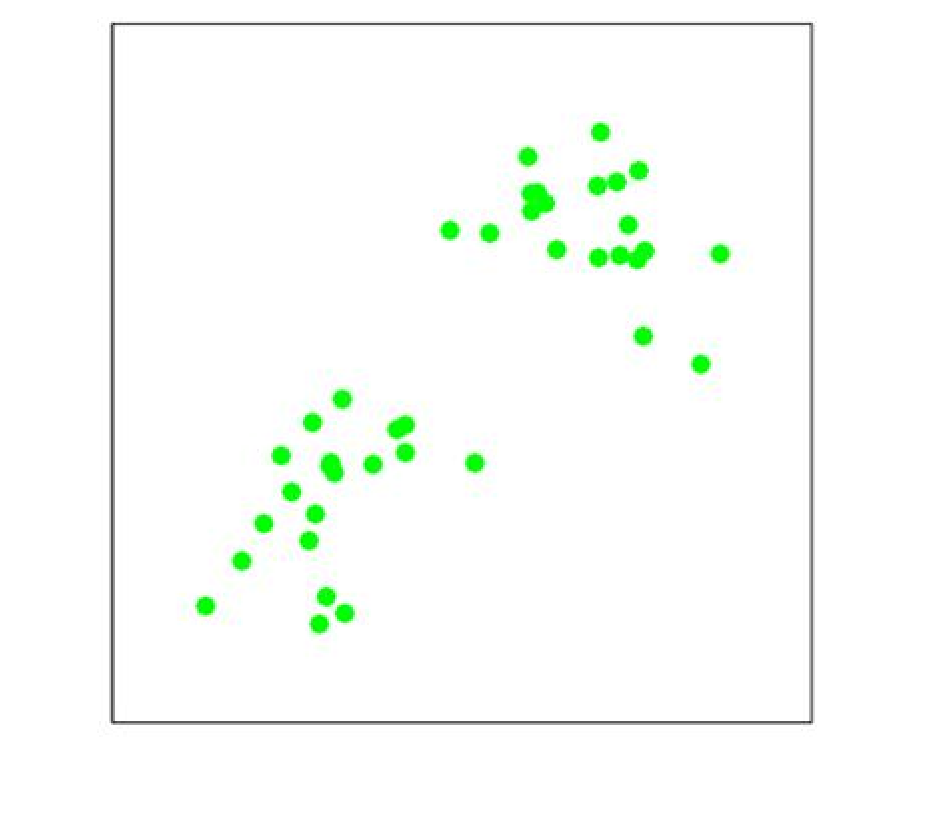
\includegraphics[width=\textwidth]{kmeans/kmeans1.eps}
    \caption{}
    \label{}
  \end{subfigure}
  \hfill
  \begin{subfigure}[b]{0.3\textwidth}
    \centering
    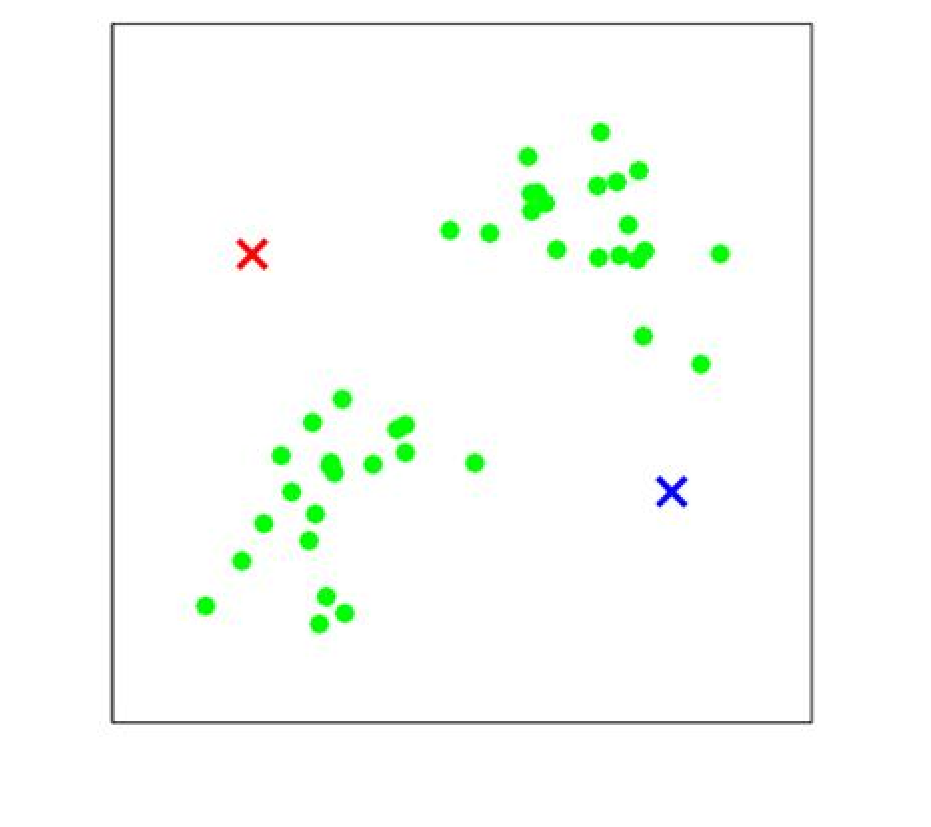
\includegraphics[width=\textwidth]{kmeans/kmeans2.eps}
    \caption{}
    \label{}
  \end{subfigure}
  \hfill
  \begin{subfigure}[b]{0.3\textwidth}
    \centering
    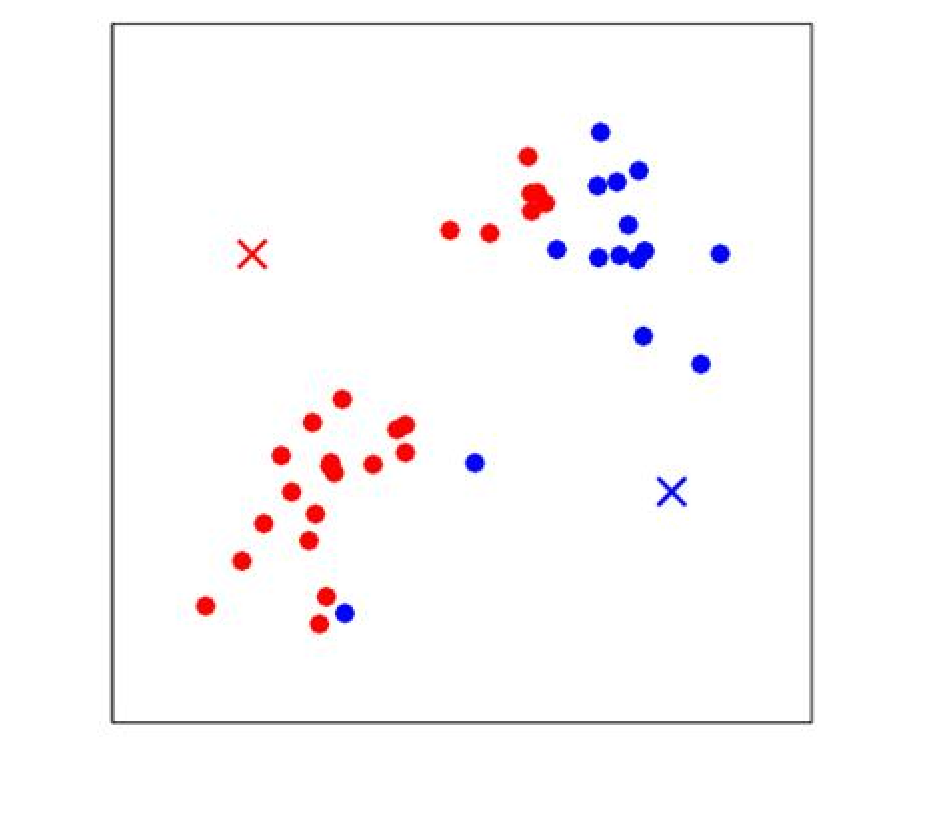
\includegraphics[width=\textwidth]{kmeans/kmeans3.eps}
    \caption{}
    \label{}
  \end{subfigure}
  \hfill
  \begin{subfigure}[b]{0.3\textwidth}
    \centering
    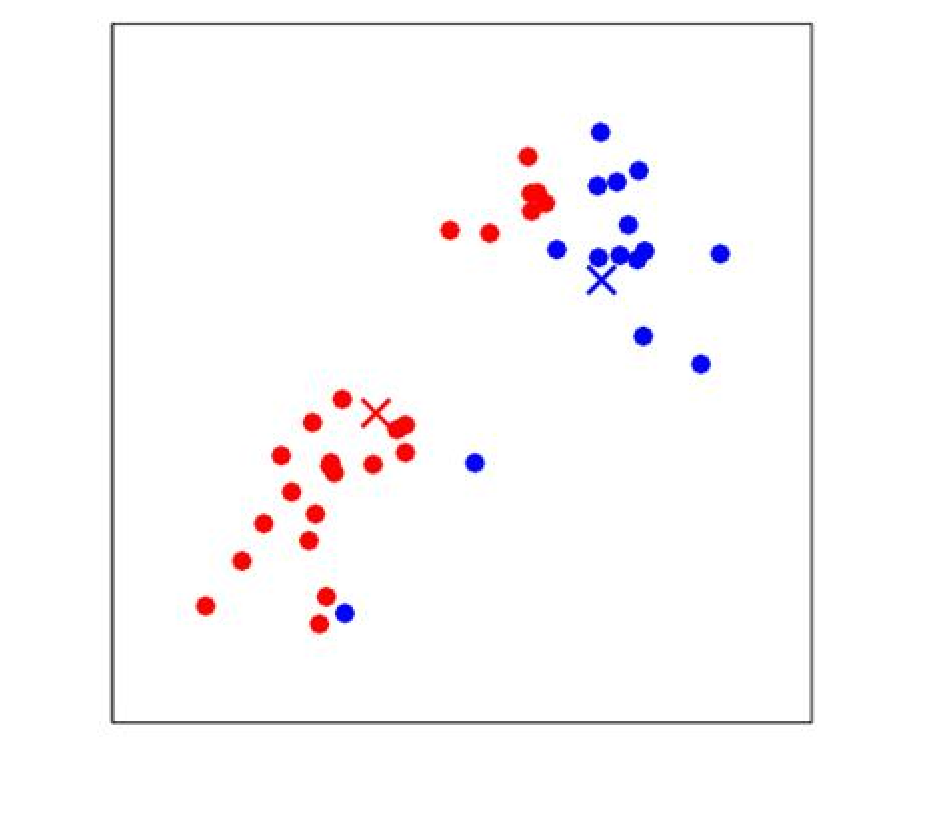
\includegraphics[width=\textwidth]{kmeans/kmeans4.eps}
    \caption{}
    \label{}
  \end{subfigure}
  \hfill
  \begin{subfigure}[b]{0.3\textwidth}
    \centering
    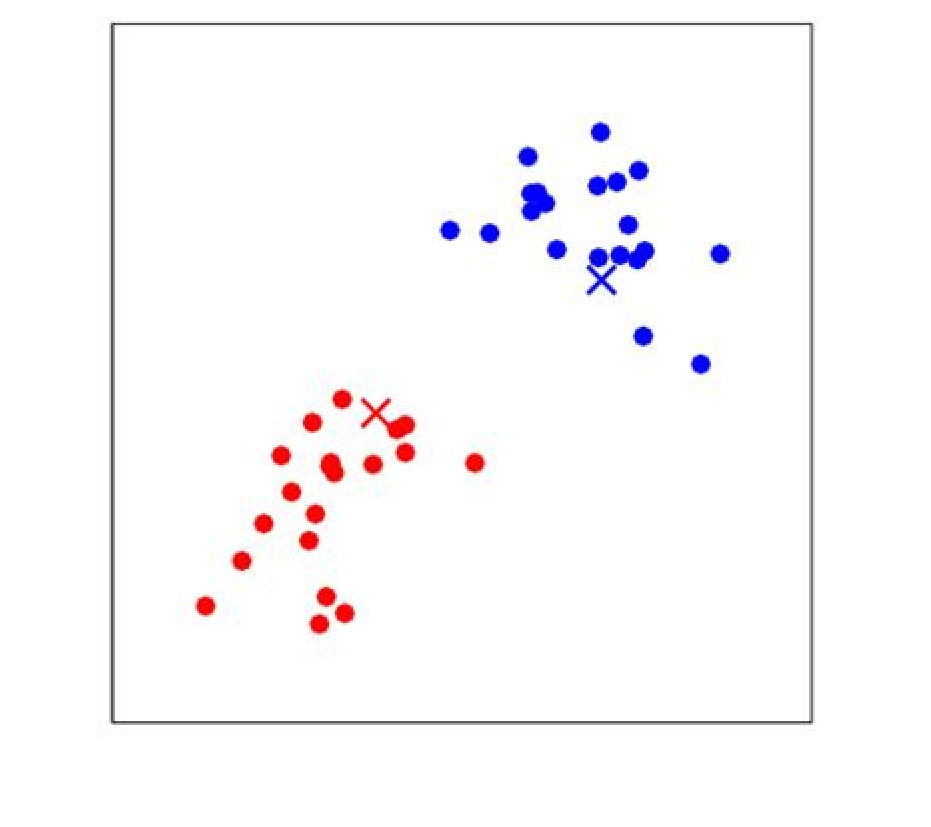
\includegraphics[width=\textwidth]{kmeans/kmeans5.eps}
    \caption{}
    \label{}
  \end{subfigure}
  \hfill
  \begin{subfigure}[b]{0.3\textwidth}
    \centering
    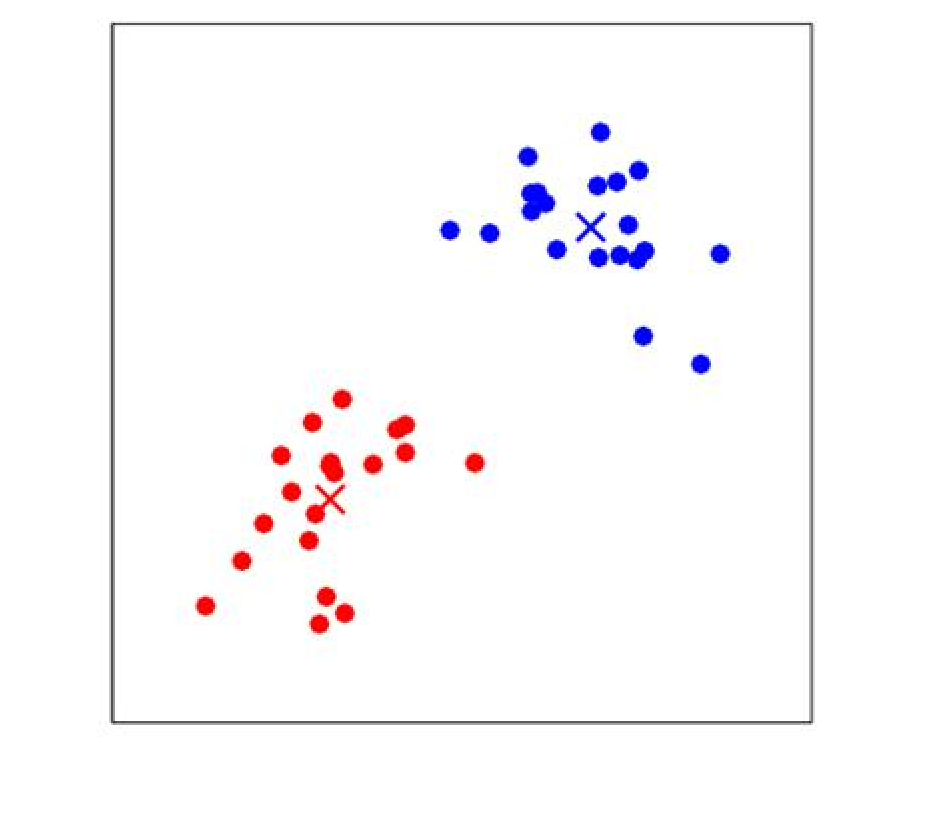
\includegraphics[width=\textwidth]{kmeans/kmeans6.eps}
    \caption{}
    \label{}
  \end{subfigure}
  \caption{K-means algorithm. Training examples are shown as dots, and cluster
  centroids are shown as crosses.  (a) Original dataset. (b) Random initial cluster
  centroids (in this instance, not chosen to be equal to two training examples). (c-f) Illustration of running
  two iterations of $k$-means.  In each iteration, we assign each training example 
  to the closest cluster centroid (shown by ``painting'' the training examples 
  the same color as the cluster centroid to which is assigned); then we move
  each cluster centroid to the mean of the points assigned to it.  (Best viewed in color.) 
  Images courtesy Michael Jordan.}
  \label{}
\end{figure}

% \begin{figure}[t]

%   \centering
%   \subfigure[]{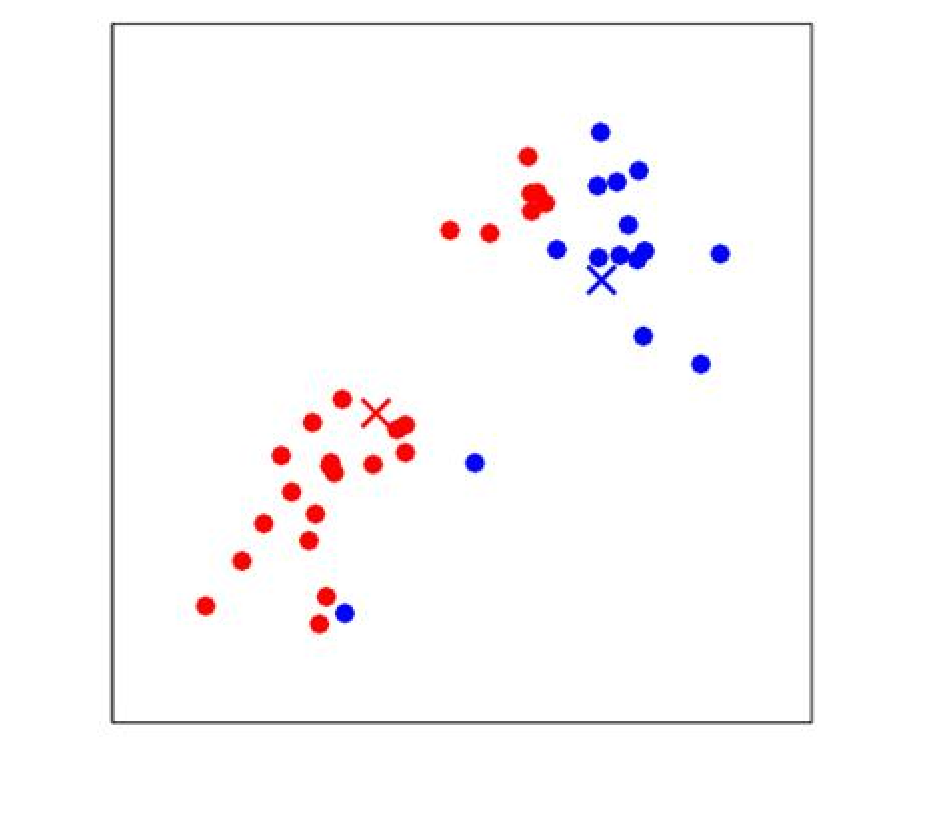
\includegraphics[width=0.24\textwidth]{kmeans/kmeans4.eps}}
%   \subfigure[]{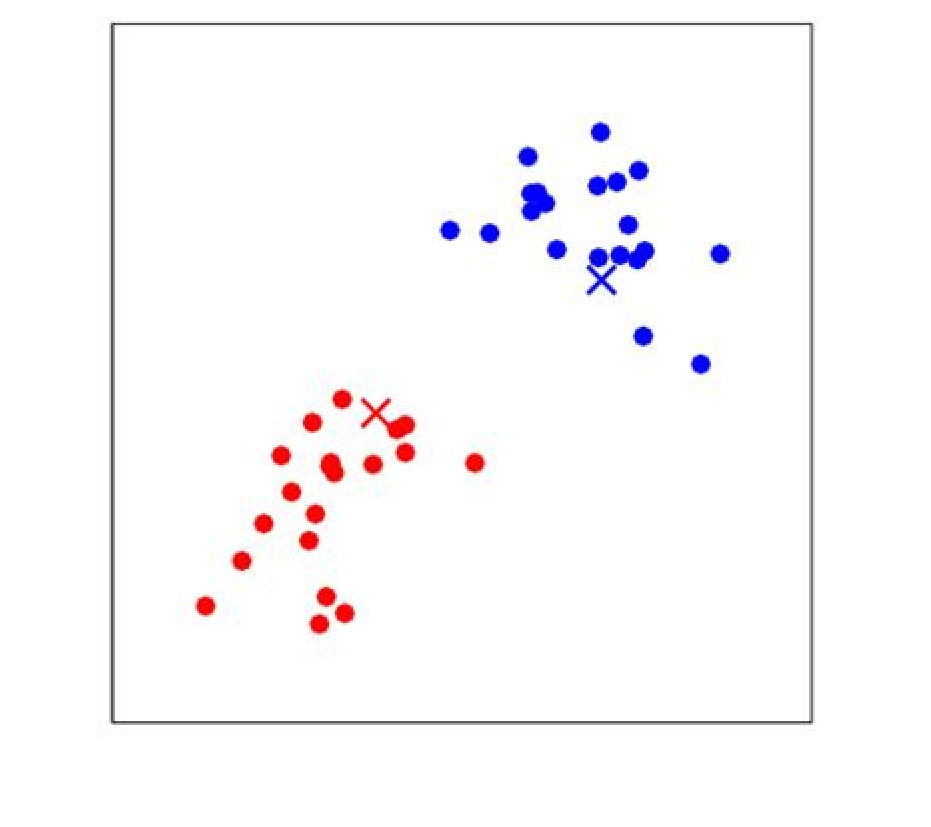
\includegraphics[width=0.24\textwidth]{kmeans/kmeans5.eps}} 
%   \subfigure[]{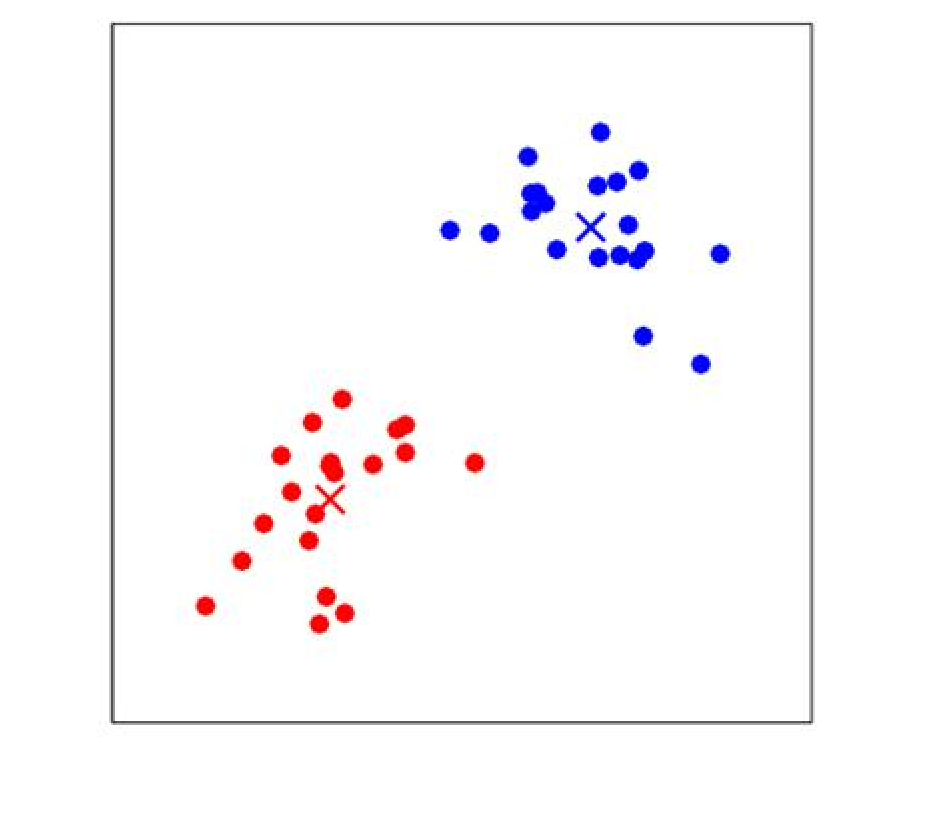
\includegraphics[width=0.24\textwidth]{kmeans/kmeans6.eps}}
%   % 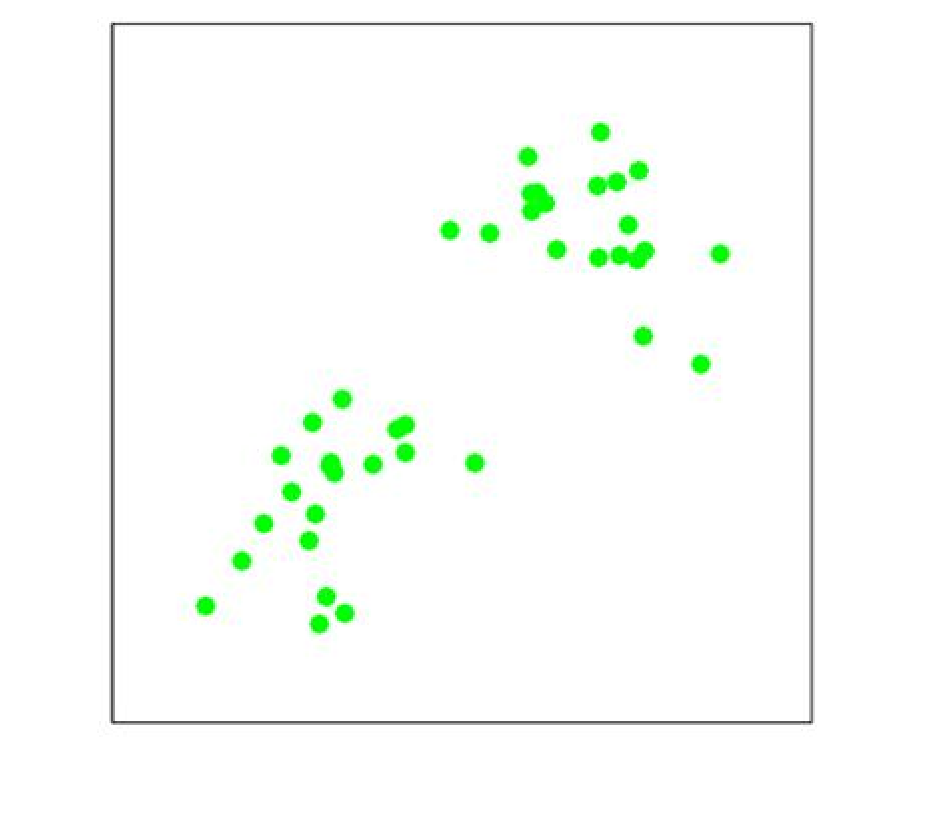
\includegraphics[width=.3\textwidth]{kmeans/kmeans1.eps}\hfill
%   % 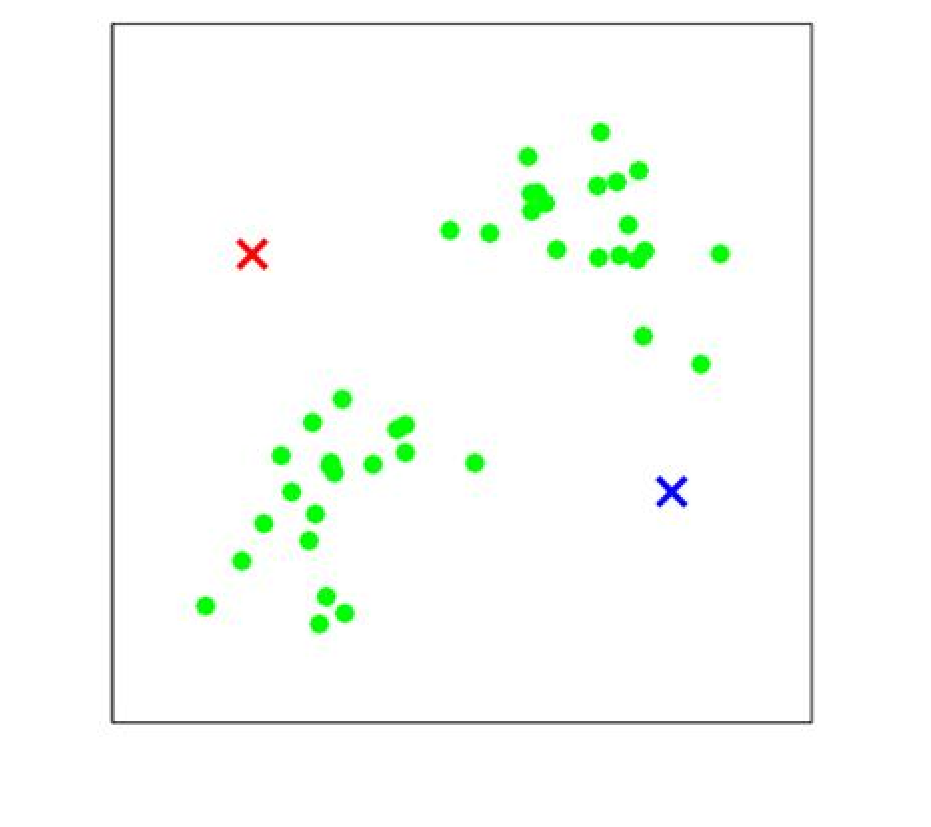
\includegraphics[width=.3\textwidth]{kmeans/kmeans2.eps}\hfill
%   % 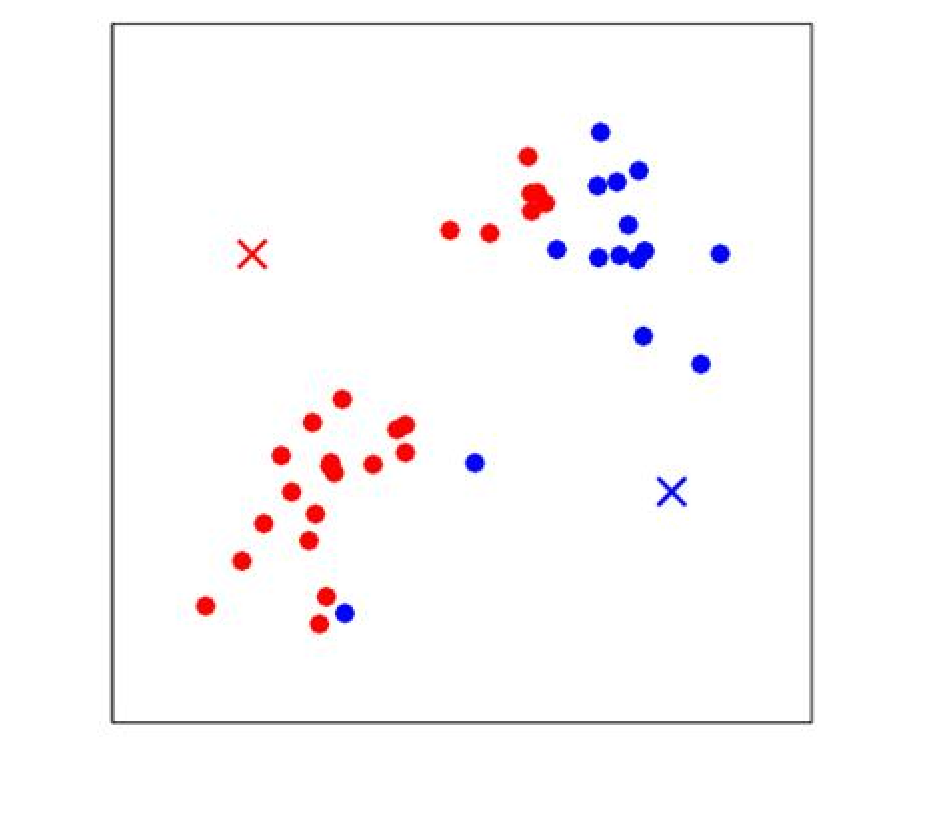
\includegraphics[width=.3\textwidth]{kmeans/kmeans3.eps}
%   \caption{(d) (e) (f)}
%   \label{fig-kmeans-2}
%   % \caption{default}
%   % \label{fig:figure3}
% \end{figure}


% \vskip 0.1in
% \threefigboxdef{kmeans/kmeans4.eps}{kmeans/kmeans5.eps}{kmeans/kmeans6.eps} 
% \end{figure}

Is the $k$-means algorithm guaranteed to converge?  Yes it is, in a certain sense.
In particular, let us define the {\bf distortion function} to be: 
\[
J(c, \mu) = \sum_{i=1}^\nexp ||x^{(i)} - \mu_{c^{(i)}}||^2
\]
Thus, $J$ measures the sum of squared distances between each training example $\xsi$
and the cluster centroid $\mu_{c^{(i)}}$ to which it has been assigned.  It can
be shown that $k$-means is exactly coordinate descent on $J$.  Specifically, the inner-loop
of $k$-means repeatedly minimizes $J$ with respect to $c$ while holding $\mu$ fixed, and then
minimizes $J$ with respect to $\mu$ while holding $c$ fixed.
Thus, $J$ must
monotonically decrease, and the value of $J$ must converge.  (Usually, this implies
that $c$ and $\mu$ will converge too.  In theory, it is possible
for $k$-means to oscillate between a few different clusterings---i.e., a few different
values for $c$ and/or $\mu$---that have exactly
the same value of $J$, but this almost never happens in practice.)

The distortion function $J$ is a non-convex function, and so coordinate 
descent on $J$ is not guaranteed to converge to the global minimum.  In other words, $k$-means
can be susceptible to local optima.  Very often $k$-means will work fine and come up with
very good clusterings despite this.  But if you are worried about getting stuck in bad 
local minima, one common thing to do is run $k$-means many times (using different
random initial values for the cluster centroids $\mu_j$).  Then, out of all the
different clusterings found, pick the one that gives the lowest distortion $J(c,\mu)$. 

\end{document}


